% LREC-COLING 2024 Example; 
% LREC Is now using templates similar to the ACL ones. 
\documentclass[10pt, a4paper]{article}

\usepackage[final]{lrec-coling2024} % this is the new style
\usepackage{amsmath}
\usepackage{amsfonts}
\usepackage{float}
\usepackage{tablefootnote}

\DeclareMathSymbol{\mhyphen}{\mathord}{AMSa}{"39}

\title{Comparing News Framing of Migration Crises using Zero-Shot Classification}

\name{Nikola Ivačič$^{1}$, Matthew Purver$^{1,2}$, Fabienne Lind$^{3}$,
\\ {\bf \large Hajo Boomgaarden$^{3}$, Veronika Bajt$^{4}$, Senja Pollak$^{1}$}} 

\address{$^{1}$Jožef Stefan Institute\\ Jamova 39, 1000 Ljubljana, Slovenia\\$^{2}$School of Electronic Engineering and Computer Science\\ Queen Mary University of London, \\ London E1 4NS, UK \\
$^{3}$University of Vienna, Department of Communication, \\ Computational Communication Science Lab \\ Kolingasse 14-16, 1090 Vienna, Austria\\ $^{4}$Peace Institute \\ Metelkova 6, 1000 Ljubljana, Slovenia. \\
         \{nikola.ivacic, matthew.purver, senja.pollak\}@ijs.si \\ \{fabienne.lind, hajo.boomgaarden\}@univie.ac.at \\veronika.bajt@mirovni-institut.si}

%Nikola Ivačič nikola.ivacic@ijs.si
%Matthew Purver matthew.purver@ijs.si
%Fabienne Lind fabienne.lind@univie.ac.at
%Hajo Boomgaarden hajo.boomgaarden@univie.ac.at
%Veronika Bajt Veronika.Bajt@mirovni-institut.si
%Senja Pollak senja.pollak@ijs.si

%School of Electronic Engineering and Computer Science, Queen Mary University of London, London E1 4NS, UK
%Jožef Stefan Institute, Jamova 39, 1000 Ljubljana, Slovenia
%University of Vienna, Department of Communication, Computational Communication Science Lab, Kolingasse 14-16, 1090 %Vienna, Austria.
%Institute for Contemporary Social and Political Studies, Metelkova 6, 1000 Ljubljana, Slovenia.

\abstract{
We present an experiment on classifying news frames in a language unseen by the learner, using zero-shot cross-lingual transfer learning. 
We used two pre-trained multilingual Transformer Encoder neural network models and tested with four specific news frames, investigating two approaches to the resulting multi-label task:
Binary Relevance (treating each frame independently) and Label Power-set (predicting each possible combination of frames). 
We train our classifiers on an available annotated multilingual migration news dataset and test on an unseen Slovene language migration news corpus, first evaluating performance and then using the classifiers to analyse how media framed the news during the periods of Syria and Ukraine conflict-related migrations.
 \\ \newline \Keywords{Transfer learning, Zero-shot classification, News Framing, Migrations} }

\begin{document}

\maketitleabstract

\section{Introduction}
\label{sec:introduction}

News articles can portray topics by means of different styles of presentations and by emphasising different facets of the topic.
News framing describes the selection of particular aspects of topics, people or events and rendering them salient to promote a particular interpretation, evaluation, and/or solution \citep{entman_framing_1993, entman_cascading_2003, de_vreese2005}.
Social scientists have long sought to computationally measure these frames, with researchers comparing various machine learning methods~\citep{burscher_2014, eisele_2023, lind_2021}, despite the varying and informal definitions of framing. Although computational methods for detecting framing have been extensively explored~\citep{ali-hassan-2022-survey}, they have recently gained significant attention in NLP research~\citep{piskorski-etal-2023-semeval, eisele_2023}, indicating a notable advancement in zero-shot computational framing research~\citep{wu-etal-2023-sheffieldveraai, reiter-haas-etal-2023-mcpt}.

We aimed to analyse and compare the framing of news in Slovenia during two distinct European migration waves, one triggered by the war in Syria and the other by the war in Ukraine. Both events saw a considerable rise of migrants entering the European Union \citep{KogovsekBajt, niemann}; yet the migrant groups differed markedly in terms of cultural and ethnic background. Both the context causing migration as well as cultural factors may play into how news media frame the migration issue during these two episodes (for an overview of the literature on media and migration, see \citealp{eberl_2018}). In the Slovenian context, \citealp{bucarRucman} discusses how migrants from different migration waves were treated differently by authorities, the local population and the media. Therefore, we generally hypothesise that the way news was framed in Slovenia varied between these periods, which will also be reflected in a quantitative computational study. A related question was addressed by \citealp{caporusso_2024}, who investigated how the dehumanisation aspects of migrant dehumanisation changed in Slovenian newspapers during the Ukrainian and Syrian periods.

We used a manually annotated news corpus \citeplanguageresource{IEGQ1B_2020} developed for the REMINDER project\footnote{\url{https://www.reminder-project.eu/}} to train the multilingual frame classifiers.
This corpus consisted of migration news articles in seven languages - yet not our target language, Slovene - and was manually annotated with four issue-specific frames. These frames have been frequently studied in European news coverage of migration \citep{eberl_2018, chouliaraki_2017}.

For the classification, we chose two multilingual pre-trained Transformer Encoder \cite{devlin2018, conneau2019} models and fine-tuned them on the migration corpus for multi-label classification.
While recent methods employing a contrastive learning approach exist~\citep{reiter-haas-etal-2023-mcpt, liao-etal-2023-marseclipse}, we utilised classical techniques for our study.
We used two transformation methods to tackle multi-label classification problems: Binary Relevance and Label Power-set (\citealp{ganda_survey_2018}; see Section~\ref{sec:methodology}).

The Zero-shot technique, first used in classification tasks with a target to predict new unseen classes~\citep{chang2008zero, larochelle2008zero, palatucci2009zero}, has been applied in many NLP tasks and settings, including cross-lingual model transfer in which task-specific annotations in one language are used to fine-tune the model for evaluation in another language~\citep{pires2019multilingual}. 
Zero-shot cross-lingual model transfer has been demonstrated from Slovene to Croatian language on other tasks, e.g.\ offensive language detection \citep{pelicon2020zero} and for genre identification in Slovene texts \citep{kuzman2023chatgpt}.

We aimed to analyse Slovene news, but as no annotated training set exists, we tested whether zero-shot transfer would work.
Consequently, we created a Slovene news corpus on migration for both periods, applied fine-tuned models to predict news framing, and analysed the results.

In summary, the contributions of this paper are two-fold: a) the development and testing of a multilingual news frames classifier for migration texts and b) the comparative analysis of Slovene news from two different migration-related periods. 

\section{Data Description}
\label{sec:data_descr}
The following section presents the two corpora used in our experiments: The manually annotated REMINDER migration corpus and our Slovenia migration news corpus.

\subsection{The REMINDER migration corpus}
The manually annotated REMINDER corpus is a randomly selected sample of migration-related news articles published between January 2000 and December 2017.
It contains 6,475 news articles from seven countries: Germany, Hungary, Poland, Romania, Spain, Sweden and the UK, with 925 samples per country. 
Each news article is marked with four labels showing whether an article contains aspects related to a specific migration-related frame.
The labels were created by seven native speakers who coded the articles in their original language. 
These coders underwent joint training to ensure a shared comprehension of the four frame concepts. 
Intercoder reliability was evaluated.
Those labels are coded as one if an article references the respective frame or zero if it does not.
The labels in question are as follows:
\begin{itemize}
  \item Economy: Does the article refer to economy/budget-related aspects of migration?
  \item Labour market: Does the article refer to labour market-related aspects of migration?
  \item Welfare: Does the article refer to welfare-related aspects of migration?
  \item Security: Does the article refer to security-related aspects of migrants/migration?
\end{itemize}
We filtered the corpus, removing double-occurring symbol characters that could negatively impact sub-word tokenisation and have no information value.

\begin{figure}[!ht]
\begin{center}
    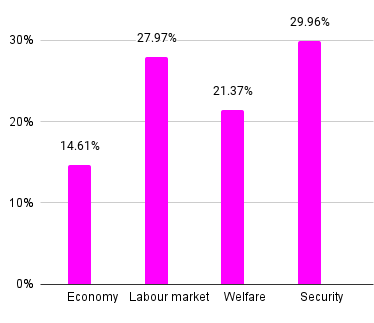
\includegraphics[scale=0.5]{label-freq.png} 
    \caption{A bar for each label illustrates the Percentage of samples labelled with each frame.}
    \label{fig.1}
\end{center}
\end{figure}

\begin{figure}[!ht]
\begin{center}
    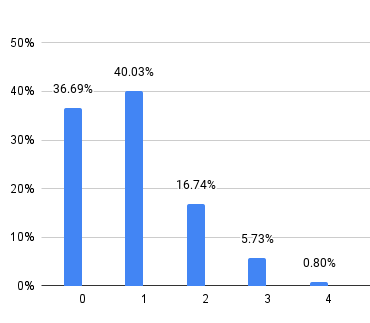
\includegraphics[scale=0.5]{num-labels-per-sample.png} 
    \caption{Distribution of the number of labels per sample, across all samples}
    \label{fig.2}
\end{center}
\end{figure}

In our examination of a corpus, we discovered two significant imbalances. 
Firstly, the distribution of individual labels within the corpus is uneven; for example, the label Economy is noticeably less frequent than other labels (see Figure~\ref{fig.1}).
Secondly, there is a significant variation in the number of labels assigned to each sample, with multiple frame combinations less frequent than 0 or single frame labels, indicating an imbalance in label distribution per sample (see Figure~\ref{fig.2}). 
%\hl{MP: FIg 2 doesn't show this, though; it just shows that multiple frame combinations are less frequent than 0 or single frame labels}
%Nikola TODO: reformulate

Adding to these challenges is the issue that the most common label set is the empty set; this introduces a considerable bias towards unlabelled samples.
Upon examining the label distribution, considering only single-label sets (which represent the largest group by label count), it is clear that the Security label appears far more frequently than any other in this context (see Figure~\ref{fig.3}).
In contrast, the Economy label set is notably smaller, highlighting a significant disparity in label representation.


\begin{figure}[!ht]
\begin{center}
    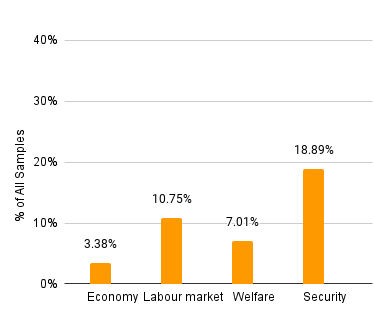
\includegraphics[scale=0.5]{single-label-freq.png} 
    \caption{The distribution of single label sets across all samples}
    \label{fig.3}
\end{center}
\end{figure}

\subsection{The Slovene migration corpus}
For the transfer learning task, we collected the Slovene news corpus from 29 online news media outlets (see Appendix~\ref{subsec:slo_media_outlets}). 
In this study, the selected media outlets encompassed major players and representative local media, ensuring a comprehensive analysis of the media landscape.
We used a set of Slovene word prefixes frequently used in migration-related articles (shown in Table~\ref{tab:search_prefixes}) and two distinct periods for the Syria and Ukraine migration crisis: August 2015 until April 2016 and  February 2022 until March 2023.

\begin{table}[!ht]
  \begin{center}
  \resizebox{\linewidth}{!}{
  {\renewcommand{\arraystretch}{1.2}% for the vertical padding
    \begin{tabular}{|l|l|}
        \hline
        \textbf{Search Prefixes}&English Translation \\
        \hline
        begunec, begunc, begunk, beguns&refugee\\
        \hline
        migracij, migrant, imigra&migration, migrant, emigrant\\
        \hline
        prebežni, pribežni&migration, migrant\\
        \hline
        azil&asylum\\
        \hline
    \end{tabular}}}
    \caption{Search prefixes used for Slovene corpus construction.}
    \label{tab:search_prefixes}
 \end{center}
\end{table}
These periods were selected to reflect the timeframe of increased migration from conflict areas to Europe and Slovenia. 
On the one hand, in the summer of 2015, the Balkans migration route from the Middle East to Turkey, Greece, Macedonia, Serbia, and Hungary also turned through Croatia and Slovenia (after Hungary closed its borders). 
According to the official Slovenian Police statistics, almost 400,000 migrants entered Slovenia between September 2015 and January 2016, most just passing through. On the other hand, following Russia's invasion of Ukraine on 24 February 2022, the European Union activated a Temporary Protection Directive that has been in effect in Slovenia since March 2022. More than 8,000 Ukrainian citizens have since received temporary protection in Slovenia. Both events resulted in pronounced media reporting about migration. 

These search criteria yielded almost equal dataset sizes for the 2015/16 and the 2022/23 periods: 8617 and 8586, respectively.

Next, we manually annotated a small sample of 100 articles to act as an evaluation set for classification accuracy.
We used our classifier to predict label values on the Slovene corpus and randomly selected equal numbers of positive and negative values for each of the four labels.
We took 50 articles from both periods, resulting in 100 articles; these were then manually annotated to obtain a Slovene classification test set. Manual labelling was carried out by a single annotator following the coding instructions for the REMINDER corpus project.
%\hl{MP: likely reviewer question: how many annotators, what was the inter-annotator agreement, etc}

\section{Methodology}
\label{sec:methodology}
%\hl{SP: You can split this section to methods and evaluation metrics, and then name the next section Results}
We employed BERT Multilingual Cased \citep{devlin2018} (BERTmc) and XLM-Roberta-base \citep{conneau2019} (XLMRb) pre-retrained Transformer models from HuggingFace \cite{wolf-etal-2020-transformers}. We fine-tuned the models on the REMINDER corpus using two distinct combinations of news article fields: including the body with the title (T+B) and excluding the title (B).

Migration-related media frames were modelled as a multi-label classification problem, as multiple or zero frames may occur in the same news article.
The small label count enabled the use of HuggingFace's built-in classification capabilities without the need for a custom neural network classification head to address the multi-label problem.
This was achieved through the implementation of two problem transformation methods:
\begin{itemize}
  \item Binary Relevance (BinRel), where we independently fine-tuned one transformer model per label.
  \item Label Power-set (LPSet), where we fine-tuned each label combination as a separate class.
\end{itemize}

We conducted a 10-fold cross-validation on the REMINDER corpus for six combinations involving two pre-trained models, two fields, and two transformation methods. Then, we compared the outcomes with those of the majority label-set and random classifiers.

The concluding phase involved classifying the Slovene migration corpus, choosing and manually annotating a small set of 100 articles, and then examining the outcomes. 
%Manual labelling was carried out by a single annotator following the guidelines established by the REMINDER corpus project.

In this work, we did not perform hyper-parameter optimisation; all the models are fine-tuned using the default set of hyper-parameters in the Transformers library, optimised for a large selection of common NLP tasks.
More precisely, we used:
\begin{itemize}\itemsep=0pt
  \item AdamW optimiser with a learning rate of $2e-5$.
  \item Weight decay set to 0.01 for regularisation.
  \item Training for a maximum of 20 epochs.
  \item Batch size of 24.
  \item Maximum length of 512 sub-word tokens.
  \item Best model selection based on the validation set micro F1-score.
\end{itemize}

\section{Evaluation}
\label{sec:evaluation}
Here, we explain the measures used to assess our models, followed by an analysis of the fine-tuning results on the REMINDER corpus. 
Finally, we evaluate the Slovene language zero-shot classification, examining the effectiveness of our approach across different scenarios.

\subsection{Evaluation Metrics}
\label{subsec:evaluation_metrics}
Following the work of \citealp{Tsoumakas2010, madjarov2012}, we employed two categories of metrics:
\begin{itemize}\itemsep=0pt
    \item Example-based metrics, namely Hamming Loss and Accuracy, to assess the differences between the actual and predicted label sets across all samples.
    \item Label-based metrics, including Precision, Recall, and Macro-F1, to examine performance averaged across all labels.
\end{itemize}
We have selected the macro averaged Label-based metrics treating all labels of equal importance to have a better understanding of the model's performance on each label individually (see Appendices for micro-averaged results and formulas).

For a baseline comparison, we selected three straightforward classifiers: the $Majority\;\emptyset$ classifier, which assigns no labels to all samples; the $Majority\; L_1$, which labels all samples with the most common single label (Security); and the $Random$ classifier, which assigns labels based on the overall distribution of label-sets.

\subsection{Fine-Tuning Results}
\label{subsec:fine_tuning_results}

This section will present the classification results of fine-tuning Transformer Encoder models across multiple languages on the REMINDER migration corpus.

The results in Table~\ref{tab:fine_tuning_example_results} and Table~\ref{tab:fine_tuning_label_results} show the manually annotated corpus 10-fold cross-validated classifier performance. 
Examining the results, we can see that the XLM-Roberta pre-trained models and the Binary Relevance problem transformation method outperform BERT and Label Power-set in both metrics categories.
For the best model, we can see that almost $60\%$ of example label sets are exactly matched while $13\%$ of example-label pair is misclassified (see Appendix~\ref{subsec:formulas} for details).
\begin{table}[H]
  \begin{center}
  \resizebox{\linewidth}{!}{
  {\renewcommand{\arraystretch}{1.2}% for the vertical padding
  \begin{tabular}{lllll}
        \hline
        Model & Method & Field & Accuracy & Hamming Loss \\ 
        \hline
        XLMRb & BinRel & B & \(\mbox{\boldmath$0.587$} \pm 0.026\) & \(\mbox{\boldmath$0.131$} \pm 0.011\) \\
        XLMRb & BinRel & T+B & \(0.575 \pm 0.028\) & \(0.133 \pm 0.011\) \\
        XLMRb & LPSet & B & \(0.571 \pm 0.023\) & \(0.137 \pm 0.009\) \\
        XLMRb & LPSet & T+B & \(0.572 \pm 0.016\) & \(0.138 \pm 0.009\) \\
        BERTmc & BinRel & B & \(0.557 \pm 0.021\) & \(0.143 \pm 0.008\) \\
        BERTmc & BinRel & T+B & \(0.548 \pm 0.025\) & \(0.144 \pm 0.009\) \\
        BERTmc & LPSet & B & \(0.531 \pm 0.020\) & \(0.155 \pm 0.009\) \\
        BERTmc & LPSet & T+B & \(0.524 \pm 0.021\) & \(0.159 \pm 0.008\) \\
        \hline
        \multicolumn{5}{c}{Baseline models}\\
        \hline
        \multicolumn{3}{l}{Majority $\emptyset$} & \(0.367\) & \(0.235\) \\
        \multicolumn{3}{l}{Majority $L_1$} & \(0.189\) & \(0.335\) \\
        \multicolumn{3}{l}{Random} & \(0.192\) & \(0.355\) \\
        \hline
  \end{tabular}}}
  \caption{Example-based classifier performance - shows the pre-trained model used for fine-tuning, followed by a problem transformation method, selected article fields for training, classification accuracy (higher is better), and Hamming loss (lower is better). The results are compared to baseline models (the no-label, the most common label, and the random classifier).}
  \label{tab:fine_tuning_example_results}
  \end{center}
\end{table}

It is evident that the choice of training fields from news articles has a minimal effect on classifier performance across both metric categories. 
Adding a title to the body negatively affects performance, suggesting that titles alone offer limited informational value.

\begin{table}[H]
\begin{center}
  \resizebox{\linewidth}{!}{
  {\renewcommand{\arraystretch}{1.2}% for the vertical padding
    \begin{tabular}{llllll}
        \hline
        Model & Method & Fields & Macro F1 & Precision & Recall \\ 
        \hline
        XLMRb & BinRel & B & \(\mbox{\boldmath$0.709$} \pm 0.019\) & \(\mbox{\boldmath$0.714$} \pm 0.027\) & \(0.707 \pm 0.026\) \\
        XLMRb & BinRel & T+B & \(0.705 \pm 0.016\) & \(0.705 \pm 0.030\) & \(\mbox{\boldmath$0.709$} \pm 0.026\) \\
        XLMRb & LPSet & B & \(0.686 \pm 0.023\) & \(0.706 \pm 0.030\) & \(0.670 \pm 0.030\) \\
        XLMRb & LPSet & T+B & \(0.683 \pm 0.017\) & \(0.698 \pm 0.029\) & \(0.672 \pm 0.025\) \\
        BERTmc & BinRel & B & \(0.674 \pm 0.017\) & \(0.687 \pm 0.020\) & \(0.663 \pm 0.025\) \\
        BERTmc & BinRel & T+B & \(0.675 \pm 0.016\) & \(0.686 \pm 0.021\) & \(0.669 \pm 0.022\) \\
        BERTmc & LPSet & B & \(0.649 \pm 0.017\) & \(0.657 \pm 0.028\) & \(0.648 \pm 0.032\) \\
        BERTmc & LPSet & T+B & \(0.642 \pm 0.015\) & \(0.648 \pm 0.028\) & \(0.643 \pm 0.029\) \\
        \hline
        \multicolumn{6}{c}{Baseline models}\\
        \hline
        \multicolumn{3}{l}{Majority $L_1$} & \(0.115\) & \(0.075\) & \(0.250\) \\
        \multicolumn{3}{l}{Random} & \(0.231\) & \(0.230\) & \(0.232\) \\
        \hline
    \end{tabular}}}
    \caption{Label-based classifier performance - shows the pre-trained model used for fine-tuning, followed by a problem transformation method, selected article fields for training, macro F1 score, macro precision and macro recall (higher is better for all three values). The results are compared to the baseline models (the most common label and the random classifier).}
    \label{tab:fine_tuning_label_results}
\end{center}
\end{table}

All models that underwent fine-tuning significantly surpassed the performance of the baseline models.\footnote{The baseline classifier's performance excludes the $Majority\;\emptyset$ classifier for label-based metrics, as it does not generate any true positives.}
Their performance is also consistent regarding micro-averaged scores (see Appendix~\ref{subsec:micro_fine_tuning_results}).

\subsection{Zero-Shot Results}
\label{subsec:zero_shot_results}

Next, we needed to assess how well the classifier performed on the unseen Slovene language.
We tested classifier performance on the 100 manually annotated Slovenian corpus articles.
Although the model's performance fell short of expectations, it still surpassed the baseline on both categories of evaluation, indicating some level of effectiveness.
%We can see (Table~\ref{tab:zeroshot_example_results}) that the model performs poorly if we look at the Hamming loss and the model's classification accuracy.

\begin{table}[H]
\begin{center}
  \resizebox{\linewidth}{!}{
  {\renewcommand{\arraystretch}{1.2}% for the vertical padding
    \begin{tabular}{lllll}
        \hline
        Model & Method & Fields & Accuracy & Hamming Loss \\ 
        \hline
        XLMRb & BinRel & B & \(0.340\) & \(0.255\) \\
        XLMRb & BinRel & T+B & \(\mbox{\boldmath$0.370$}\) & \(0.253\) \\
        XLMRb & LPSet & B & \(0.340\) & \(\mbox{\boldmath$0.250$}\) \\
        XLMRb & LPSet & T+B & \(0.330\) & \(0.255\) \\
        \hline
        \multicolumn{5}{c}{Baseline models}\\
        \hline
        \multicolumn{3}{l}{Majority $\emptyset$} & \(0.210\) & \(0.308\)\\
        \multicolumn{3}{l}{Majority $L_1$} & \(0.270\) & \(0.273\) \\
        \multicolumn{3}{l}{Random} & \(0.160\) & \(0.353\) \\
        \hline
    \end{tabular}}}
\caption{Example-based Zero-Shot classifier performance - shows the pre-trained model used, followed by a problem transformation method, selected article fields for training, classification accuracy (higher is better), and Hamming loss (lower is better). The results are compared to baseline models (the no-label, the most common label, and the random classifier).}
\label{tab:zeroshot_example_results}
\end{center}
\end{table}

It is noticeable that the poor recall values of the classifier impact the overall performance of the label-based metrics.

\begin{table}[H]
\begin{center}
  \resizebox{\linewidth}{!}{
  {\renewcommand{\arraystretch}{1.2}% for the vertical padding
    \begin{tabular}{llllll}
        \hline
        Model & Method & Fields & Macro F1 & Macro P & Macro R \\ 
        \hline
        XLMRb & BinRel & B & \(0.422\) & \(0.605\) & \(0.341\) \\
        XLMRb & BinRel & T+B & \(0.445\) & \(0.616\) & \(0.367\) \\
        XLMRb & LPSet & B & \(\mbox{\boldmath$0.466$}\) & \(\mbox{\boldmath$0.640$}\) & \(\mbox{\boldmath$0.412$}\) \\
        XLMRb & LPSet & T+B & \(0.461\) & \(0.595\) & \(0.403\) \\
        \hline
        \multicolumn{6}{c}{Baseline models}\\
        \hline
        \multicolumn{3}{l}{Majority $L_1$} & \(0.182\) & \(0.143\) & \(0.250\) \\
        \multicolumn{3}{l}{Random} & \(0.267\) & \(0.275\) & \(0.265\) \\
        \hline
    \end{tabular}}}
    \caption{Label-based Zero-Shot classifier performance - shows the pre-trained model used, followed by a problem transformation method, selected article fields for training, macro F1 score, macro precision and macro recall (higher is better for all three values). The results are compared to the baseline models (the most common label and the random classifier).}
    \label{tab:zeroshot_label_results}
\end{center}
\end{table}

\subsection{Zero-Shot Predictions}
\label{subsec:zero_shot_predictions}

Lastly, we proceeded to run predictions on the entire Slovene corpus with the best models from fine-tuning and zero-shot evaluation for both periods and examined distributions of the individual labels.

%\hl{SP, MP do-review:}
All predictions show consistent results regarding prevailing frame labels for each period regardless of model selection (see Table~\ref{tab:predictions}). We wanted to assess if the difference in predictions of our models for the two periods is significant.
The difference between the predicted distributions for the two periods is statistically significant, with a $\chi^2$ test showing a p-value nearly zero, well below the standard threshold $0.05$ for all three selected models.
%\hl{SP: not fully clear, explain a bit more and add reference to the table with results: All predictions show consistent results regarding prevailing frame labels for each period.}
%The chi-square p-value for the prediction results is nearly zero, falling well below the significance threshold ($\alpha = 0.05$).\hl{SP: which table, add ref.? Table 6 shows raw frequencies, so I am unsure if we can claim it. Is it for another table?} 


%\hl{SP: I changed the paragraph above with Veronika's text. However, I referred to Fig 4 and not tab: predictions. Please check if we can delete the sentence below, and check the comments edited there }
\begin{table}[H]
\begin{center}
  \resizebox{\linewidth}{!}{
  {\renewcommand{\arraystretch}{1.2}% for the vertical padding
    \begin{tabular}{lllccccc}
        \hline
        Model & Method & Fields & Period & Economy & Labour M. & Welfare & Security \\ 
        \hline
        \multicolumn{8}{c}{Best Fine-Tuning model predictions}\\
        \hline
        XLMRb & BinRel & B & Syria & 796 & 590 & 973 & 2023 \\
        XLMRb & BinRel & B & Ukraine & 517 & 895 & 1218 & 1661 \\
        \hline
        \multicolumn{8}{c}{Best Zero-Shot model predictions}\\
        \hline
        XLMRb & BinRel & T+B & Syria & 890 & 753 & 1230 & 2022 \\
        XLMRb & BinRel & T+B & Ukraine & 600 & 1182 & 1434 & 1697 \\
        XLMRb & LPSet & B & Syria & 1161 & 870 & 950 & 1908 \\
        XLMRb & LPSet & B & Ukraine & 718 & 1272 & 1183 & 1797 \\
        \hline
    \end{tabular}}}
    \caption{Best model predictions - shows the pre-trained model used, followed by a problem transformation method, selected article fields for training, number of predicted labels for Economy, Labour Market, Welfare and Security.}
    \label{tab:predictions}
\end{center}
\end{table}

Figure \ref{fig.4} shows that the security frame is by far the most prevalent in both corpora, corroborating the existing research about migration, in general, becoming regarded as a security risk \citep{Palidda, bajt2019, pajnikRibac}. When comparing the distributions across the two subcorpora, it also shows that security has been a more exposed frame in media coverage of Middle Eastern migration to Europe than that of Ukrainians (see also sociological research by \citealp{bucarRucman}). Moreover, Muslims are stereotypically portrayed as dangerous as the idea of violent Muslims corresponds to racialised views of young Middle Eastern men as terrorists \citep{kundnani}. Syrian refugees have thus been treated as a threat also in Slovenian media \citep{thiele}. 

On the other hand, the labour market and welfare aspects were more prevalent during the Ukraine migration wave. This pattern may be in line with what could be expected, given that the cultural and ethnic background of migrants from the Middle East tends to reproduce discourses that refer to alleged security issues posed by such migration \citep{sambaraju_2023}. 
By contrast, it is possible that the vast and very quick increase of migrants from Ukraine has posed challenges in terms of welfare provision for these migrants in particular. The prevalence of the welfare frame and the absence of the security frame also mirrors the findings for the UK press in their reporting on Ukrainian refugees \citep{roman_2020}. 

\begin{figure}[H]
\begin{center}
    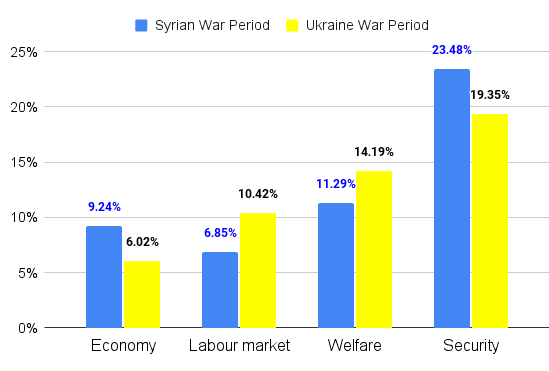
\includegraphics[scale=0.4]{pred-sl-body-labels.png} 
    \caption{Final Zero-Shot prediction results on a complete Slovene migration news corpus obtained with the best model from the fine-tuning results.}
    \label{fig.4}
\end{center}
\end{figure}

\section{Conclusion}
We tested several approaches for news frame classification on the REMINDER multilingual migration news corpus. We discovered that employing a binary relevance problem transformation approach combined with the XLM-Roberta-base pre-trained model yields the most effective results. The model was then evaluated on a small Slovene sample, where zero-shot performance is around $0.37$ regarding classification accuracy.

Although our model performance is clearly suboptimal, and individual labels and absolute percentages will be errorful, we can still draw some conclusions from relative distributions and comparisons across settings. Given this, we take our results as tentative support for the hypothesis that the portrayal of migration by the news media varied across the two periods in its focus on the economy, labour market, welfare, and security. Moreover, our analysis suggests that economic and security issues were more prominent in media reports on migration during the Middle East conflict than during the Ukraine war.
Likewise, it is apparent that labour market and welfare concerns received more emphasis in discussions of migration during the period of the Ukraine war. 


Overall, it is also interesting to see that security framing, in line with the REMINDER results, remains the most prominent news frame detected in the Slovenian corpus, independent of context and type of migration \citep{stormback_2021}.


In our pursuit of enhancing the classification model, which is crucial for a more reliable interpretation of results, future efforts will focus on several key areas of improvement.  
Firstly,  we plan to pre-train the models further using the Slovene migration corpus, specifically targeting the masked language modelling task. 
This approach aims to deepen the models' understanding of context and nuances regarding migration within the Slovene language. 
Secondly, to mitigate the effects of possible truncation, which can lead to the loss of vital information in longer texts, we intend to explore the use of models designed for handling extended sequences, such as ToBERT~\citep{pappagari2019hierarchical}, Longformer~\citep{beltagy2020longformer}, Big Bird~\citep{zaheer2021big}. Lastly, we want to incorporate contrastive learning techniques tailored for Few-Shot scenarios \citep{reiter-haas-etal-2023-mcpt, liao-etal-2023-marseclipse}. 
This innovative approach could enhance the model's ability to learn from a limited number of examples, thereby improving its performance in classifying new, unseen data with minimal additional input.
Additionally, we plan to investigate the use of generative model approaches, not only to improve classification accuracy potentially but also to enrich the training corpus. 

\section{Acknowledgements}
This work was supported by the Slovenian Research Agency grants via the core research programmes Knowledge Technologies (P2-0103) and the projects Computer-assisted multilingual news discourse analysis with contextual embeddings (J6-2581), Embeddings-based techniques for Media Monitoring Applications (L2-50070) and Hate Speech in Contemporary Conceptualizations of Nationalism, Racism, Gender and Migration (J5-3102). 

We would also like to thank Špela Rot for her contribution to the frame labelling of manually annotated Slovene corpora.

\section{Limitations}
The classification performance is above the baselines but still far from optimal.
Consequently, any analysis and resultant conclusions regarding framing within the Slovene corpus must be approached cautiously and can only be considered tentative support for the hypotheses.


\nocite{*}
\section{References}
\label{sec:reference}
\subsection{Bibliographical References}
\label{subsec:bib_reference}

\bibliographystyle{lrec-coling2024-natbib}
\bibliography{news_framing}

\subsection{Language Resource References}
\label{subsec:res_reference}
\bibliographystylelanguageresource{lrec-coling2024-natbib}
\bibliographylanguageresource{languageresource}


\section{Appendices}
\label{sec:appendices}
\appendix
\addcontentsline{toc}{section}{Appendices}
\renewcommand{\thesubsection}{\Alph{subsection}}

\subsection{Formulas}
\label{subsec:formulas}
In this section, we use $N$ for the number of samples, $L$ for the number of labels, $y_i$ for an individual example label set, and $\hat{y_i}$ for the predicted example label set.

For the example-based evaluation, we used
\begin{itemize}
  \item Subset accuracy:
    \begin{equation*}
      Accuracy = \frac{1}{N}\sum_{i=1}^{N}I( y_i = \hat{y_i})
    \end{equation*}
    where  $I(true) = 1$ and $I(false) = 0$
  \item Hamming loss:
    \begin{equation*}
      Hamming\mhyphen Loss = \frac{1}{N \cdot L}\sum_{i=1}^{N}\sum_{j=1}^{L}{xor(y_{i_j},\hat{y_{i_j}})}
    \end{equation*}
\end{itemize}

For the label-based macro-averaged evaluation, we used:

    \begin{equation*}
      Precision_{macro} = \frac{1}{L}\sum_{i=1}^{L}\frac{TP_i}{TP_i + FP_i}
    \end{equation*}

    \begin{equation*}
      Recall_{macro} = \frac{1}{L}\sum_{i=1}^{L}\frac{TP_i}{TP_i + FN_i}
    \end{equation*}

For the label-based micro-averaged evaluation, we used:

    \begin{equation*}
      Precision_{micro} = \frac{\sum_{i=1}^{L} TP_i}{\sum_{i=1}^{L} (TP_i + FP_i)}
    \end{equation*}

    \begin{equation*}
      Recall_{micro} = \frac{\sum_{i=1}^{L} TP_i}{\sum_{i=1}^{L} (TP_i + FN_i)}
    \end{equation*}

In both cases the $F_1\mhyphen score$ can be computed as follows:
    \begin{equation*}
      F_1\mhyphen score = 2  \cdot \frac{Precision \cdot Recall}{Precision +  Recall}
    \end{equation*}




\subsection{Micro-averaged Fine-Tuning Results}
\label{subsec:micro_fine_tuning_results}

\begin{table}[H]
\begin{center}
  \resizebox{\linewidth}{!}{
  {\renewcommand{\arraystretch}{1.2}% for the vertical padding
    \begin{tabular}{lllccc}
        \hline
        Model & Method & Field & Micro F1 & Precision & Recall \\ 
        \hline
        XLMRb & BinRel & B & \(\mbox{\boldmath$0.721$} \pm 0.020\) & \(\mbox{\boldmath$0.723$} \pm 0.026\) & \(\mbox{\boldmath$0.720$} \pm 0.028\) \\
        XLMRb & BinRel & T+B & \(0.719 \pm 0.016\) & \(0.717 \pm 0.030\) & \(0.722 \pm 0.023\) \\
        XLMRb & LPSet & B & \(0.702 \pm 0.021\) & \(0.719 \pm 0.030\) & \(0.686 \pm 0.024\) \\
        XLMRb & LPSet & T+B & \(0.702 \pm 0.018\) & \(0.714 \pm 0.028\) & \(0.692 \pm 0.025\) \\
        BERTmc & BinRel & B & \(0.690 \pm 0.017\) & \(0.703 \pm 0.018\) & \(0.678 \pm 0.027\) \\
        BERTmc & BinRel & T+B & \(0.690 \pm 0.016\) & \(0.696 \pm 0.023\) & \(0.685 \pm 0.021\) \\
        BERTmc & LPSet & B & \(0.669 \pm 0.015\) & \(0.572 \pm 0.027\) & \(0.667 \pm 0.031\) \\
        BERTmc & LPSet & T+B & \(0.663 \pm 0.017\) & \(0.661 \pm 0.026\) & \(0.531 \pm 0.032\) \\
        \hline
        \multicolumn{6}{c}{Baseline}\\
        \hline
        \multicolumn{3}{l}{Majority $L_1$} & \(\mbox{\boldmath$0.309$}\) & \(\mbox{\boldmath$0.300$}\) & \(\mbox{\boldmath$0.319$}\) \\
        \multicolumn{3}{l}{Random} & $0.247$ & $0.246$ & $0.248$ \\
        \hline
    \end{tabular}}}
    \caption{Label-based Zero-Shot classifier performance - shows the pre-trained model used, followed by a problem transformation method, selected article fields for training, micro F1 score, micro precision and micro recall.}
    \label{tab:fine_tuning_label_results_micro}
\end{center}
\end{table}


\subsection{Micro-averaged Zero-Shot Results}
\label{subsec:micro_zero_shot_results}

\begin{table}[H]
\begin{center}
  \resizebox{\linewidth}{!}{
  {\renewcommand{\arraystretch}{1.2}% for the vertical padding
    \begin{tabular}{lllccc}
        \hline
        Model & Method & Fields & micro F1 & micro P & micro R \\ 
        \hline
        XLMRb & BinRel & B & \(0.457\) & \(\mbox{\boldmath$0.662$}\) & \(0.350\) \\
        XLMRb & BinRel & T+B & \(0.471\) & \(\mbox{\boldmath$0.662$}\) & \(0.366\) \\
        XLMRb & LPSet & B & \(\mbox{\boldmath$0.490$}\) & \(0.658\) & \(0.390\) \\
        XLMRb & LPSet & T+B & \(\mbox{\boldmath$0.490$}\) & \(0.636\) & \(\mbox{\boldmath$0.398$}\) \\
        \hline
        \multicolumn{6}{c}{Baseline models}\\
        \hline
        \multicolumn{3}{l}{Majority $L_1$} & \(\mbox{\boldmath$0.511$}\) & \(\mbox{\boldmath$0.570$}\) & \(\mbox{\boldmath$0.463$}\) \\
        \multicolumn{3}{l}{Random} & \(0.410\) & \(0.422\) & \(0.398\) \\
        \hline
    \end{tabular}}}
    \caption{Label-based Zero-Shot classifier performance - shows the pre-trained model used, followed by a problem transformation method, selected article fields for training, micro F1 score, micro precision and micro recall}
    \label{tab:zeroshot_label_results_micro}
\end{center}
\end{table}

\subsection{Slovene corpus media outlets}
\label{subsec:slo_media_outlets}
\begin{table}[H]
\begin{center}
  \resizebox{\linewidth}{!}{
  {\renewcommand{\arraystretch}{1.2}% for the vertical padding
  \begin{tabular}{lll}
        \textbf{id}&\textbf{name}&\textbf{url}\\
    \hline
        10&24ur.com&https://www.24ur.com/\\
        20&Celje.info&https://www.celje.info/\\
        30&Delo.si&https://www.delo.si/\\
        40&Demokracija.si&https://demokracija.si/\\
        50&Dnevnik.si&https://www.dnevnik.si/\\
        60&Dolenjskilist.si&https://www.dolenjskilist.si/\\
        70&Domovina.je&https://www.domovina.je/\\
        80&Druzina.si&https://www.druzina.si/\\
        90&Ekipa.svet24.si&https://ekipa.svet24.si/\\
        100&Gorenjskiglas.si&https://www.gorenjskiglas.si/\\
        110&Kozjansko.info&https://kozjansko.info/\\
        120&Lokalec.si&https://lokalec.si/\\
        130&Mladina.si&https://www.mladina.si/\\
        140&N1info.si&https://n1info.si\\
        150&Necenzurirano.si&https://necenzurirano.si/\\
        160&Nova24tv.si&https://nova24tv.si/\\
        170&Novice.svet24.si&https://novice.svet24.si/\\
        180&Novitednik.si&https://www.novitednik.si/\\
        190&Politikis.si&http://www.politikis.si/\\
        200&Primorske.si&https://www.primorske.si/\\
        210&Primorski.eu&https://www.primorski.eu/\\
        220&Prlekija-on.net&https://www.prlekija-on.net/\\
        230&Reporter.si&https://reporter.si/\\
        240&Rtvslo.si&https://www.rtvslo.si/\\
        250&Siol.net&https://siol.net/\\
        260&Slovenskenovice.si&https://www.slovenskenovice.si/\\
        270&Vecer.com&https://www.vecer.com/\\
        280&Vestnik.si&https://vestnik.si/\\
        290&Zurnal24.si&https://www.zurnal24.si/\\
    \hline
  \end{tabular}}}
  \caption{Slovene news media sources. Showing corpus media identifier, media source name, and media source URL}
  \label{tab:slo_sources}
\end{center}
\end{table}

\end{document}

%%% Local Variables:
%%% mode: latex
%%% TeX-master: t
%%% End:
